\documentclass[dvipdfmx]{jarticle}
\pagestyle{empty}
\usepackage{tikz}
\usetikzlibrary{shapes,calc}
\begin{document}
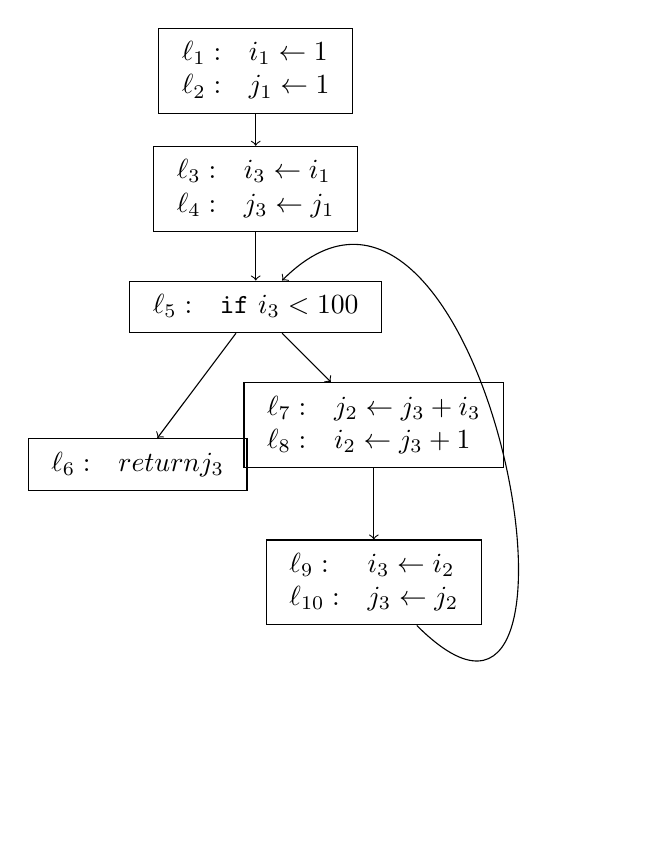
\begin{tikzpicture}
\node[draw] (N1) at (0,0) {$\begin{array}{ll}
    \ell_1: & i_1\leftarrow 1\\
    \ell_2: & j_1\leftarrow 1\end{array}$};
\node[draw] (N12) at (0,-1.5) {$\begin{array}{ll}
    \ell_3: & i_3\leftarrow i_1\\
    \ell_4: & j_3\leftarrow j_1
\end{array}$};
\node[draw] (N2) at (0,-3) {$\begin{array}{ll}
    \ell_5: & \texttt{if}\ i_3<100
\end{array}$};
\node[draw] (N3) at (-1.5,-5) {$\begin{array}{ll}
    \ell_6: & return j_3
\end{array}$};
\node[draw] (N4) at (1.5,-4.5) {$\begin{array}{ll}
    \ell_7: & j_2\leftarrow j_3+i_3\\
    \ell_8: & i_2\leftarrow j_3+1\end{array}$};
\node[draw] (N42) at (1.5,-6.5) {$\begin{array}{ll}
    \ell_9: & i_3\leftarrow i_2\\
    \ell_{10}: & j_3\leftarrow j_2
\end{array}$};
\path[->] (N1) edge (N12) (N12) edge (N2) (N2) edge (N3) (N2) edge (N4) (N4) edge (N42);
\path[->] (N42) edge [out=315,in=45,looseness=2.0] (N2);
\end{tikzpicture}

\end{document}